\section{DAPHNE Front-End}
\label{sec:system}

DAPHNE is the front-end system for the Horizontal Drift Photon Detection System at DUNE. The signals from the XArapucas are amplified by a Cold Electronics system inside the TPC. These signals are transported by differential pairs to the warm side and digitized by DAPHNE. A trigger algorithm does the first discrimination of the signals in the FPGA. The Acquired data is sent to the DAQ system to Deploy in the LArSoft data frame.

\subsection{DAPHNE design}
\label{sec:requirements}

The design of the DAPHNE board is based on the Mu2e board (Cita) developed at Fermilab, from which it keeps the same architecture with an FPGA and a microcontroller, the core of the power supply, and the use of an analog front-end chip (AFE)~\cite{IEEE_Ref1:afe5808amanual}. Apart from the mentioned similarities, DAPHNE includes modifications concerning Mu2e, like the use of a different FPGA and microcontroller family, a total redesign of the voltage regulators block, and the upgraded model AFE5808A, among others. The development group introduced these changes to accomplish the requirements needed to achieve the PDS readout characteristics from the technical design report:

\begin{itemize}
    \item Signal-to-noise > 4 			\cite{} (SP-PDS-14)
    \item < 1 us time resolution 		\cite{} (SP-FD-4)
    \item < 1 kHZ dark noise rate 		\cite{} (SP-PDS-15)
    \item 2000 PE dynamic range 		\cite{} (SP-PDS-16)
\end{itemize}

Many FD level specifications drive DAPHNE characteristics. That affects signal size sensitivity, signal to noise (SNR), timing resolution, event size and data transfer limits, power needs and dissipation limits, channel density, channel count, and cost:

\begin{itemize}
\item 40 Channel granularity
\item 14 bit resolution
\item 65 MSPS
\item SNR > 2
\item Power supply for the active ganging
%\item Increase the effective bandwidth of the output ($4 \times 3.7Gb/s$)
\end{itemize}

A general overview of the main components and architecture of the board is presented in the figure~\ref{fig:DAPHNEBlocksScheme}

\begin{figure}[htbp]
\centering % \begin{center}/\end{center} takes some additional vertical space
%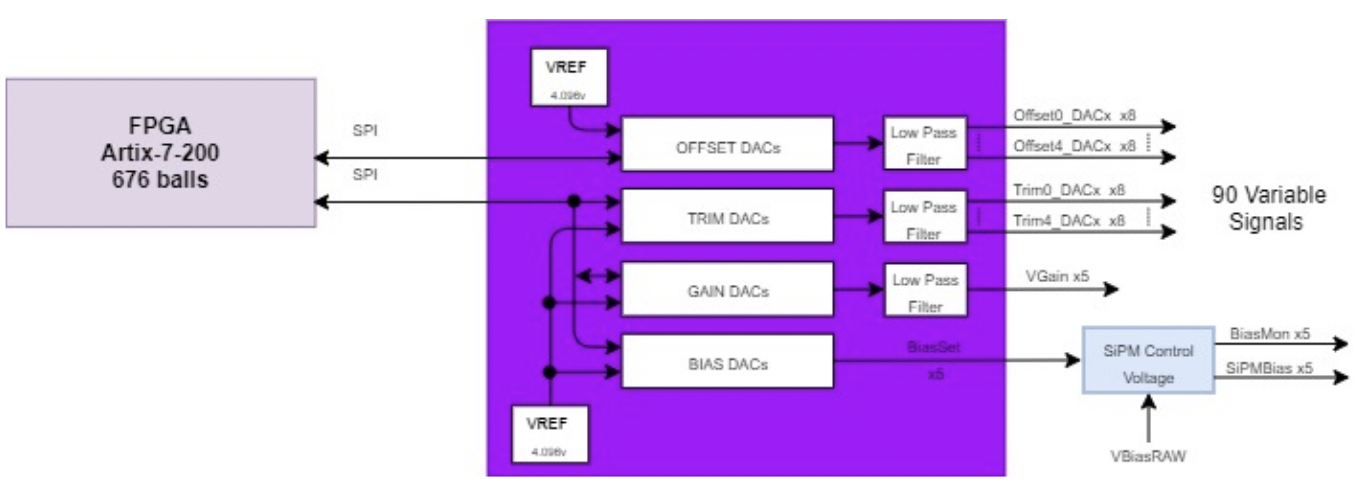
\includegraphics[width=.8\textwidth,trim=30 110 0 0,clip]{Images/BiasControl.png}
%\qquad
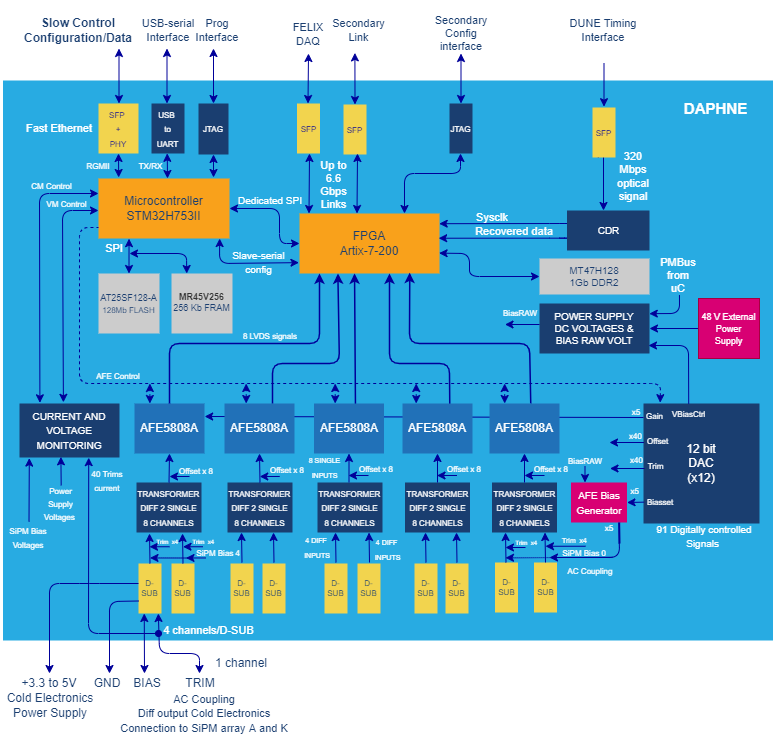
\includegraphics[width=1.\textwidth,origin=c,angle=0]{Images/Block_Diagram_DAPHNEV1_rev2.png}
% "\includegraphics" from the "graphicx" permits to crop (trim+clip)
% and rotate (angle) and image (and much more)
\caption{\label{fig:DAPHNEBlocksScheme} DAPHNE general scheme.}
\end{figure}

The first stage of signal conditioning is based on differential to single transformers. In this stage is, embedded the SiPMs bias voltage generator and control; more details are presented in section~\ref{sec:interfaces}  

The unipolar signals are digitized using the Analog Front End chips. There are 5 AFEs, eight channels each, for 40 channels. The AFEs are arrays of programmable active or passive impedances, a low noise amplification, an external voltage controller attenuator, a programmable gain amplification, a low pass filter, and 14 bits analog to digital converter. The control of all these elements is a task of the micro-controller embedded in DAPHNE.

The FPGA reads the digital data generated by the AFEs with a frequency of $62.5MHz$. In addition, the FPGA can select an event using an internal trigger and save the data that will be streamed by optical fibers to the DAQ system at a rate of $4.8Gbps$ using an external hardware and software protocol called FELIX (Cita) 


A more detailed description of the primary digital devices implemented in the DAPHNE board is presented in the following.

\subsubsection{AFE5808A}

The AFE5808A is an analog front-end (AFE) intended to be used in the digitization of analog signals \cite{afe5808a} for applications based on doppler effect. In the case of DAPHNE, its special characteristics fit according to experiment requirements, in few words 14 bits of data resolution, a sample rate of 62.5 Msps, embedded filtering techniques like Low pass filtering and high pass filtering, and finally a pre amplifier stage before digitizing the data.

There are two important interfaces to operate the AFE's

\begin{itemize}
\item Serial Peripheral Interface (SPI): Configuration via SPI. It is a standard serial interface used to write on configure registers, in order to enable, disable or configure the special characteristics present in this device. 

\item Data output: The interface it's an LVDS interface connected directly to the FPGA. Each AFE transmits to the FPGA a total of 10 LVDS signals; 8 LVDS signals corresponding to each analog input channel, 1 LVDS signal corresponding to the frame clock and 1 LVDS signal for the digital clock.
\end{itemize}

In the case of the AFE, DAPHNE uses 5 of such devices, eight channels each, for a total of 40 analog channels. 

The master clock input used for each AFE is provided by the FPGA that uses five clock generators coming from the timing interface.

\subsubsection{FPGA}

The FPGA is responsible of reading the digital data coming from the 5 Analog Front End's (AFE5808A). And the last one, is the responsible of processing 8 analog channels coming from the Cold Electronics(CE) as can be seen from the figure \ref{fig:DAPHNEBlocksScheme}.

The FPGA used on DAPHNE is the Xilinx Artix-7, model XC7A200T-676. The FPGA supports streaming data links of 4.8 Gbps together with a communication protocol specificated by CERN~\cite{Borga:2019rwr}. In order to implement the links the use of hte  GTP transceivers on-chip is mandatory and of course a couple of external SFP connectors in order to be independent of the used medium copper or optic fiber. 

A dedicated SPI interface with the microcontroller is available for different tasks. The AFE is controlled using an SPI interface, and the data reading is allowed using an LVDS interface using a SERDES-based module~\cite{IEEE_Ref2:understanding_LVDS}. Additional FPGA functions are clock generation for AFEs and internal FPGA temperature monitoring. 

\subsubsection{Microcontroller}

The STM32H753II Cortex-M7 implementing FreeRTOS, adding new support for this STM family, is the microcontroller device used on DAPHNE. The microcontroller is responsible for monitoring and slow control tasks. The DAPHNE board provides the voltages for the photosensors ganged together accountable for detecting the scintillation light; the DAPHNE microcontroller makes the voltages and current monitoring. For slow control, a fast Ethernet link through SFP is foreseen, but an USB/UART connection is available for debugging purposes.  

Internal no volatile and external volatile memory can be used for tasks like the permanent register of operational parameters (MAC addresses, IPs, etc.) and bitstream file upload to the FPGA. A JTAG interface for programming and debugging is available in DAPHNE.



 
 








